% ============================================================
%  يُترجَم بـ XeLaTeX  (في Overleaf: Menu → Compiler → XeLaTeX)
%  الخط: Amiri (متوفر في Overleaf، أو حمّله من github.com/aliftype/amiri)
% ============================================================
\documentclass[12pt,a4paper]{article}
\usepackage[a4paper,margin=1.2cm,top=2.3cm,bottom=2.9cm,headheight=15pt,footskip=1.5cm]{geometry}
\usepackage{amsmath,amssymb}
\usepackage{icomma}
\usepackage[english,bidi=default,layout=lists]{babel}
\babelprovide[import,main]{arabic}
\babelfont{rm}[Scale=1.08]{Amiri}
\babelfont{sf}[Scale=1.08]{Amiri}
\usepackage[most]{tcolorbox}
\usepackage{tikz}
\usetikzlibrary{arrows.meta,calc,shadings,patterns}
\usepackage{array}
\usepackage{colortbl}
\usepackage{fancyhdr}
\usepackage{titlesec}
\usepackage{enumitem}
\usepackage{collcell}
\usepackage{needspace}
\usepackage{etoolbox}
\newcolumntype{C}{>{\collectcell\ar}c<{\endcollectcell}}
\pretocmd{\section}{\Needspace{15\baselineskip}}{}{}
\pretocmd{\subsection}{\Needspace{11\baselineskip}}{}{}

\definecolor{cDef}{HTML}{1F4E9C}
\definecolor{cThm}{HTML}{B3261E}
\definecolor{cRem}{HTML}{2E7D32}
\definecolor{cEx}{HTML}{C76B00}
\definecolor{cMeth}{HTML}{6A1B9A}
\definecolor{cSol}{HTML}{00695C}
\definecolor{cSec}{HTML}{1F3A68}

\titleformat{\section}{\Large\bfseries\color{cSec}}{\thesection.}{0.6em}{}[{\color{cSec!60}\titlerule[1pt]}]
\titleformat{\subsection}{\large\bfseries\color{cThm!85!black}}{\thesubsection.}{0.5em}{}
\titlespacing*{\section}{0pt}{14pt}{8pt}
\titlespacing*{\subsection}{0pt}{10pt}{5pt}
\setlength{\parindent}{0pt}
\setlength{\parskip}{4pt}
\setlist{itemsep=2pt,topsep=3pt}

\newtcolorbox{arbox}[3][]{enhanced,
  colback=#2!5,colframe=#2!80!black,arc=2mm,boxrule=0.8pt,
  left=6pt,right=6pt,top=8pt,bottom=5pt,
  fonttitle=\bfseries,coltitle=white,
  title={\foreignlanguage{arabic}{#3}},
  attach boxed title to top right={xshift=-5mm,yshift=-3mm},
  boxed title style={colback=#2!80!black,arc=1.5mm,boxrule=0pt},
  before upper={\selectlanguage{arabic}},
  before skip=8pt,after skip=8pt,breakable,#1}
\newenvironment{BOX}[2]{\begin{otherlanguage}{english}\begin{arbox}{#1}{#2}}{\end{arbox}\end{otherlanguage}}
\newenvironment{tarif}[1][تعريف]{\begin{BOX}{cDef}{#1}}{\end{BOX}}
\newenvironment{khassia}[1][خاصية]{\begin{BOX}{cThm}{#1}}{\end{BOX}}
\newenvironment{molahada}[1][ملاحظة]{\begin{BOX}{cRem}{#1}}{\end{BOX}}
\newenvironment{mithal}[1][مثال]{\begin{BOX}{cEx}{#1}}{\end{BOX}}
\newenvironment{tariqa}[1][طريقة]{\begin{BOX}{cMeth}{#1}}{\end{BOX}}

\newcounter{exo}
\newenvironment{tamrin}[1]{\stepcounter{exo}\begin{BOX}{cSec}{التمرين \theexo: #1}}{\end{BOX}}
\newenvironment{hal}{\Needspace{12\baselineskip}\begin{otherlanguage}{english}\begin{arbox}[breakable]{cSol}{حل التمرين \theexo}}{\end{arbox}\end{otherlanguage}}

\newenvironment{LTR}{\begin{otherlanguage}{english}}{\end{otherlanguage}}
\newcommand{\ar}[1]{\foreignlanguage{arabic}{#1}}

\renewcommand{\dots}{\mathinner{\ldotp\ldotp\ldotp}}
\renewcommand{\ldots}{\mathinner{\ldotp\ldotp\ldotp}}
\renewcommand{\cdots}{\mathinner{\cdotp\cdotp\cdotp}}
\newcommand{\N}{\mathbb{N}}
\newcommand{\Z}{\mathbb{Z}}
\newcommand{\D}{\mathbb{D}}
\newcommand{\Q}{\mathbb{Q}}
\newcommand{\R}{\mathbb{R}}
\newcommand{\pgcd}{\operatorname{PGCD}}
\newcommand{\ppcm}{\operatorname{PPCM}}

% \NLseg{a}{b}{[}{]} ; \NLright{a}{[} ; \NLleft{b}{]}  (interval on a number line)
\newcommand{\NLseg}[4]{\begin{LTR}\begin{tikzpicture}[baseline=-0.6ex]
 \draw[-{Stealth[length=2mm]},gray!70](0,0)--(3.4,0);
 \draw[line width=2pt,cThm!80!black](0.7,0)--(2.7,0);
 \node[cThm!80!black,font=\LARGE] at (0.7,0){$#3$};
 \node[cThm!80!black,font=\LARGE] at (2.7,0){$#4$};
 \node[below=3pt,font=\footnotesize] at (0.7,0){$#1$};
 \node[below=3pt,font=\footnotesize] at (2.7,0){$#2$};
\end{tikzpicture}\end{LTR}}
\newcommand{\NLright}[2]{\begin{LTR}\begin{tikzpicture}[baseline=-0.6ex]
 \draw[-{Stealth[length=2mm]},gray!70](0,0)--(3.4,0);
 \draw[line width=2pt,cThm!80!black](1.3,0)--(3.3,0);
 \node[cThm!80!black,font=\LARGE] at (1.3,0){$#2$};
 \node[below=3pt,font=\footnotesize] at (1.3,0){$#1$};
\end{tikzpicture}\end{LTR}}
\newcommand{\NLleft}[2]{\begin{LTR}\begin{tikzpicture}[baseline=-0.6ex]
 \draw[-{Stealth[length=2mm]},gray!70](0,0)--(3.4,0);
 \draw[line width=2pt,cThm!80!black](0.05,0)--(2.1,0);
 \node[cThm!80!black,font=\LARGE] at (2.1,0){$#2$};
 \node[below=3pt,font=\footnotesize] at (2.1,0){$#1$};
\end{tikzpicture}\end{LTR}}

% ---------- social-media icons (pure TikZ) ----------
\definecolor{cFB}{HTML}{1877F2}
\definecolor{cTG}{HTML}{229ED9}
\definecolor{cIG1}{HTML}{FEDA75}
\definecolor{cIG2}{HTML}{D62976}
\definecolor{cIG3}{HTML}{4F5BD5}
\newcommand{\fbicon}{\begin{LTR}\begin{tikzpicture}[baseline=-0.75ex,x=1em,y=1em]
 \fill[cFB] (0,0) circle (0.55);
 \node[white,inner sep=0,font=\usefont{TU}{lmss}{bx}{n}\small] at (0.04,-0.02) {f};
\end{tikzpicture}\end{LTR}}
\newcommand{\igicon}{\begin{LTR}
\begin{tikzpicture}[baseline=-0.75ex,x=1em,y=1em]
 \shade[lower left=cIG1,lower right=cIG2,upper left=cIG2,upper right=cIG3,rounded corners=0.28em] (-0.55,-0.55) rectangle (0.55,0.55);
 \draw[white,line width=0.09em,rounded corners=0.18em] (-0.36,-0.36) rectangle (0.36,0.36);
 \draw[white,line width=0.09em] (0,0) circle (0.17);
 \fill[white] (0.22,0.22) circle (0.05);
\end{tikzpicture}\end{LTR}}
\newcommand{\tgicon}{\begin{LTR}
\begin{tikzpicture}[baseline=-0.75ex,x=1em,y=1em]
 \fill[cTG] (0,0) circle (0.55);
 \fill[white] (-0.33,0.0) -- (0.32,0.27) -- (0.2,-0.3) -- (0.0,-0.15) -- (-0.08,-0.28) -- (-0.08,-0.08) -- cycle;
 \fill[cTG!70!black] (-0.08,-0.08) -- (0.25,0.2) -- (0.0,-0.15) -- (-0.08,-0.28) -- cycle;
\end{tikzpicture}\end{LTR}}
% page number: black box, white two-digit number, at the right of the social row
\newcommand{\PageBox}{\begin{LTR}\tikz[baseline=(p.base)]\node[fill=black,text=white,inner sep=2.5pt,minimum width=1.6em,minimum height=1.3em,font=\usefont{TU}{lmss}{bx}{n}\small](p){\ifnum\value{page}<10 0\fi\arabic{page}};\end{LTR}}
% visual left-to-right order: Telegram | Instagram | Facebook | page box
\newcommand{\SocialRow}{\begin{otherlanguage}{english}%
 \ar{\textbf{الأستاذ سوايسية هشام للرياضيات}}\ \tgicon\hfill
 \textbf{prof\_hicham\_math}\ \igicon\hfill
 \ar{\textbf{الأستاذ سوايسية هشام للرياضيات}}\ \fbicon\hspace{2.2em}\PageBox\end{otherlanguage}}

\pagestyle{fancy}
\fancyhf{}
\renewcommand{\headrulewidth}{0.6pt}
\renewcommand{\footrulewidth}{0.4pt}
% \SetHeader{right head: document title}{left head: level -- stream}
\newcommand{\SetHeader}[2]{%
 \fancyhead[C]{\parbox{\textwidth}{\ar{#1\hfill #2}}}%
 \fancyfoot[C]{\parbox{\textwidth}{\small\SocialRow}}}
\usepackage{tkz-tab}
\usepackage{multicol}
% variation / sign table (LTR)
\newenvironment{TAB}{\par\begin{center}\begin{LTR}\begin{tikzpicture}[scale=0.95,every node/.style={font=\small}]}{\end{tikzpicture}\end{LTR}\end{center}}
% grid + axes, clipped: \begin{GR}{xmin}{xmax}{ymin}{ymax}{unit cm}
\newenvironment{GR}[5]{\par\begin{center}\begin{LTR}\begin{tikzpicture}[x=#5cm,y=#5cm,font=\footnotesize]
 \draw[gray!25,very thin] (#1,#3) grid (#2,#4);
 \draw[-{Stealth[length=2mm]}] (#1,0)--(#2+0.3,0) node[below left]{$x$};
 \draw[-{Stealth[length=2mm]}] (0,#3)--(0,#4+0.3) node[below left]{$y$};
 \node[below left] at (0,0){$O$};
 \begin{scope}\clip (#1,#3) rectangle (#2,#4);}
{\end{scope}\end{tikzpicture}\end{LTR}\end{center}}
\newcommand{\Ticks}[2]{\foreach \t in {#1} \node[below,font=\scriptsize] at (\t,0){$\t$}; \foreach \t in {#2} \node[left,font=\scriptsize] at (0,\t){$\t$};}
\newcommand{\bx}[1]{\ensuremath{\colorbox{cDef!12}{$\displaystyle #1$}}}
\newcommand{\TwoCol}[4]{\par\begin{LTR}\noindent\begin{minipage}[t]{#1\textwidth}\selectlanguage{arabic}#2\end{minipage}\hfill\begin{minipage}[t]{#3\textwidth}\selectlanguage{arabic}#4\end{minipage}\end{LTR}\par}
\newcommand{\RL}[4]{\TwoCol{#3}{#4}{#1}{#2}}  % \RL{w1}{right content}{w2}{left content}
\newcommand{\ok}{$\textcolor{cRem}{\checkmark}$}
\newcommand{\limn}{\displaystyle\lim_{n\to+\infty}}
% sub-questions, each on its own line
\newenvironment{sq}{\begin{itemize}[leftmargin=2.4em,itemsep=3pt]}{\end{itemize}}
\newcommand{\qa}{\item[(أ)]}\newcommand{\qb}{\item[(ب)]}\newcommand{\qc}{\item[(جـ)]}\newcommand{\qd}{\item[(د)]}\newcommand{\qe}{\item[(هـ)]}
\newcommand{\pa}{\par\smallskip\textbf{(أ)} }\newcommand{\pb}{\par\smallskip\textbf{(ب)} }\newcommand{\pc}{\par\smallskip\textbf{(جـ)} }\newcommand{\pd}{\par\smallskip\textbf{(د)} }\newcommand{\pe}{\par\smallskip\textbf{(هـ)} }
\newcommand{\QQ}[1]{\par\smallskip\textbf{#1.} }
\newenvironment{tmr}{\stepcounter{exo}\begin{BOX}{cSec}{تمرين محلول \theexo}}{\end{BOX}}
\newcommand{\ABC}[3]{\\[2pt]\begin{tabular}{p{0.28\textwidth}p{0.28\textwidth}p{0.28\textwidth}}(جـ) \ #3 & (ب) \ #2 & (أ) \ #1\end{tabular}}
\pretocmd{\section}{\Needspace{24\baselineskip}}{}{}
\newtcbox{\bxtbox}{on line,colback=cDef!12,colframe=cDef!12,boxrule=0pt,arc=1pt,boxsep=0pt,left=2pt,right=2pt,top=1pt,bottom=1pt}
\newcommand{\bxtOLD}[1]{\foreignlanguage{english}{\bxtbox{\ar{#1}}}}
\usepackage{longtable}
\setlength{\LTpre}{4pt}\setlength{\LTpost}{0pt}
\newcommand{\Phase}[1]{\textbf{#1}}
\newcommand{\Fld}[2]{\textbf{#1:}\ #2}
% رأس المذكرة على نمط النموذج: إطار بعنوان «مذكرة رقم»، معلومات الحصة، ثم إطار الكفاءات
\newcommand{\ModhHead}[9]{%
\begin{LTR}
\begin{tcolorbox}[enhanced,colback=white,colframe=cThm!85!black,arc=4mm,boxrule=1pt,top=14pt,bottom=6pt,left=8pt,right=8pt,
 overlay={\node[fill=cThm!85!black,text=white,rounded corners=3mm,inner xsep=14pt,inner ysep=4pt,font=\large\bfseries] at ([yshift=0pt]frame.north){\ar{مذكرة رقم #1}};},
 before upper={\selectlanguage{arabic}}]
\begin{tabular}{@{}p{0.4\linewidth}p{0.55\linewidth}@{}}
\Fld{المستوى}{#2} & \Fld{الثانوية}{\dotfill}\\[3pt]
\Fld{المادة}{رياضيات} & \Fld{ميدان التعلم}{#3}\\[3pt]
\Fld{المدة}{#5} & \Fld{الوحدة التعلمية}{#4}\\[3pt]
\Fld{الأستاذ}{\dotfill} & \Fld{المحتوى المعرفي}{#6}\\
\end{tabular}
\end{tcolorbox}
\begin{tcolorbox}[enhanced,colback=white,colframe=cThm!85!black,arc=3mm,boxrule=0.8pt,sidebyside,sidebyside align=top,lefthand ratio=0.5,
 segmentation style={dashed,cThm!60},before upper={\selectlanguage{arabic}},before lower={\selectlanguage{arabic}}]
\textbf{الكفاءات المستهدفة:}\par #8
\tcblower
\textbf{الكفاءات القبلية:}\par #7
\end{tcolorbox}
\end{LTR}
\par\smallskip\textbf{الوسائل:} #9\par\smallskip}
\newenvironment{Sayr}{%
\begin{LTR}\renewcommand{\arraystretch}{1.25}\setlength{\tabcolsep}{4pt}\relpenalty=10000\binoppenalty=10000\tolerance=9000\emergencystretch=0.3\linewidth
\begin{longtable}{|p{0.09\textwidth}|>{\centering\arraybackslash}p{0.05\textwidth}|p{0.71\textwidth}|>{\centering\arraybackslash}p{0.09\textwidth}|}
\hline\rowcolor{cThm!12}\ar{\footnotesize\textbf{توجيهات وتعاليق}} & \ar{\footnotesize\textbf{المدة}} & \ar{\textbf{سير الحصة}} & \ar{\footnotesize\textbf{مراحل الحصة}}\\\hline\endhead
\hline\endfoot}{\end{longtable}\end{LTR}}
% سطر في الجدول: \Row{مرحلة}{سير}{مدة}{توجيهات}
\newcommand{\RaggedEnd}{\leftskip=0pt plus 1fil\relax}
\newcommand{\Row}[4]{\ar{\small #4} & \ar{#3} & \ar{\RaggedEnd #2} & \cellcolor{cThm!8}\ar{\Phase{#1}}\\\hline}

\newcommand{\Lab}[2]{\foreignlanguage{english}{\tcbox[on line,colback=#1,colframe=#1,boxrule=0pt,arc=2pt,boxsep=1pt,left=5pt,right=5pt,top=1pt,bottom=1pt]{\ar{\textcolor{white}{\textbf{#2}}}}}}
\newcommand{\Num}[1]{\foreignlanguage{english}{\tikz[baseline=(c.base)]\node[fill=cDef,text=white,inner sep=2pt,font=\footnotesize\bfseries](c){#1};}}
\newcommand{\ck}{\ensuremath{{\color{cRem}\checkmark}}}
\newenvironment{Kad}[1]{\par\smallskip\Lab{#1}}{\par}
\newcommand{\RR}[1]{\ifmmode{\color{cThm}#1}\else$\mbox{\color{cThm}#1}$\fi}
\newcommand{\T}[1]{$\mbox{\color{cDef}\bfseries #1}$}
\providecommand{\LW}[1]{{\color{cDef}#1}}
\newcommand{\bxt}[1]{}
\newenvironment{FIG}{\par\begin{center}\begin{LTR}}{\end{LTR}\end{center}}
\renewcommand{\bx}[1]{\ensuremath{\colorbox{cDef!12}{$\displaystyle\color{cThm}#1$}}}
\renewcommand{\bxt}[1]{\foreignlanguage{english}{\bxtbox{\ar{\color{cThm}#1}}}}
\newcommand{\Car}[1]{\left\{\begin{array}{l}#1\end{array}\right.}
\newcommand{\Lm}[1]{\displaystyle\lim_{x\to#1}}
\newcommand{\LDx}[3]{لدينا: $\Lm{#2}#1=\bx{#3}$ لأنّ: \quad}
\newcommand{\LD}{\par\LDx}
\newcommand{\GRS}[5]{\begin{center}\begin{LTR}\begin{tikzpicture}[x=#5cm,y=#5cm,font=\scriptsize]
 \draw[gray!25,very thin] (#1,#3) grid (#2,#4);
 \draw[-{Stealth[length=1.6mm]}] (#1,0)--(#2+0.3,0) node[below left]{$x$};
 \draw[-{Stealth[length=1.6mm]}] (0,#3)--(0,#4+0.3) node[below left]{$y$};
 \node[below left] at (0,0){$O$};}
\newcommand{\GRE}{\end{tikzpicture}\end{LTR}\end{center}}
\SetHeader{\small\bfseries\color{cSec}مذكرات محور: النهايات}{\small\color{cSec}السنة الثالثة ثانوي -- الشعب العلمية}
\newcommand{\Lmm}[2]{\displaystyle\lim_{\substack{x\to#1\\#2}}}
\newcommand{\LDy}[4]{\par لدينا: $\Lmm{#2}{#3}#1=\bx{#4}$ لأنّ: \quad}
\begin{document}
\begin{LTR}
\begin{tcolorbox}[enhanced,colback=cSec!10,colframe=cSec!40,arc=3mm,halign=center,boxrule=0.6pt,top=12pt,bottom=12pt,before upper={\selectlanguage{arabic}}]
{\color{cSec}\fontsize{24}{30}\selectfont\bfseries مذكرات محور: النهايات}\\[8pt]
{\color{cSec!80!black}\large السنة الثالثة ثانوي -- علوم تجريبية ، رياضيات ، تقني رياضي}\\[4pt]
{\color{cSec!80!black}\large 5 مذكرات -- السنة الدراسية 2026-2027}
\end{tcolorbox}
\end{LTR}
\begin{BOX}{cThm}{يتضمن هذا العمل}
\RL{0.48}{\textbf{مذكرة 24:} نهاية دالة عند مالانهاية.\par \textbf{مذكرة 25:} نهاية دالة عند عدد حقيقي.\par \textbf{مذكرة 26:} مبرهنات أولية على النهايات.}{0.48}{\textbf{مذكرة 27:} السلوك التقاربي لمنحنى دالة.\par \textbf{مذكرة 28:} العمليات على النهايات (المقارنة ، الحصر ، دالة مركبة ، النهايات المثلثية).}
\par\smallskip مراجع النشاطات والتمارين: الكتاب المدرسي للسنة الثالثة ثانوي ، الجزء الأول. \ \LW{القوانين بالأزرق} ، و\bxt{النتائج بالأحمر}.
\end{BOX}
\newpage
% =====================================================================
\ModhHead{24}{3 ع ت + 3 ت ر + 3 ر}{تحليل}{النهايات}{01 سا}{نهاية دالة عند مالانهاية}%
{\begin{itemize}\item مفاهيم أولية حول الدوال العددية.\end{itemize}}%
{\begin{itemize}\item تعيين نهاية منتهية أو غير منتهية لدالة عند $+\infty$ أو عند $-\infty$ وتفسيرها بيانيًا.\end{itemize}}%
{الكتاب المدرسي ، الأنترنت.}
\begin{Sayr}
\Row{مرحلة الانطلاق}{%
\Lab{cDef}{نهاية منتهية عند مالانهاية}\par
\Lab{cDef}{تعريف}\ $f$ دالة معرفة على مجال من الشكل $[x_0;+\infty[$ ، و $l$ عدد حقيقي.\par
القول إن نهاية $f$ عند $+\infty$ هي $l$ يعني أن كل مجال مفتوح يشمل العدد $l$ يشمل كل القيم $f(x)$ من أجل $x$ كبير بالقدر الكافي ، ونكتب:
\[\LW{\lim_{x\to+\infty}f(x)=l}\]
\GRS{-0.5}{7.5}{-0.5}{3.5}{0.6}
\fill[cDef!10] (0,1.5) rectangle (7.5,2.5);
\draw[dashed,cThm] (0,2)--(7.5,2); \draw[dashed,gray] (0,1.5)--(7.5,1.5) (0,2.5)--(7.5,2.5);
\node[left] at (0,2){$l$}; \node[left] at (0,2.5){$l+\alpha$}; \node[left] at (0,1.5){$l-\alpha$};
\draw[cDef,very thick,domain=0.4:7.4,samples=80] plot(\x,{2+1.6*sin(2*\x r)/\x});
\draw[dashed] (2.6,0)--(2.6,2.5); \node[below] at (2.6,0){$x_1$};
\node[cDef] at (6.8,3.1){$(C_f)$};
\GRE
من أجل $x>x_1$ تكون كل القيم $f(x)$ في المجال $]l-\alpha;l+\alpha[$.}{10 د}{تمثيل بياني للتعريف.}
\Row{بناء المعارف}{%
\Lab{cRem}{ملاحظة}\ نحصل على تعريف ونتيجة مماثلين عند $-\infty$.\par
\Lab{cEx}{مثال}\quad $\Lm{+\infty}\dfrac1x=\bx{0}$ \quad ؛ \quad $\Lm{-\infty}\dfrac1x=\bx{0}$\par
\Lab{cDef}{المستقيم المقارب الأفقي}\par
إذا كانت $\Lm{+\infty}f(x)=l$ (أو $\Lm{-\infty}f(x)=l$) نقول إن المستقيم ذا المعادلة $y=l$ \textbf{مستقيم مقارب أفقي} للمنحنى $(C_f)$ عند $+\infty$ (أو عند $-\infty$).
\GRS{-5}{5}{-0.5}{2.5}{0.6}
\draw[dashed,cThm,thick] (-5,2)--(5,2) node[above left]{$y=b$};
\draw[dashed,cRem,thick] (-5,0.5)--(5,0.5) node[pos=0.1,below]{$y=b^{\prime}$};
\draw[cDef,very thick,domain=-4.9:4.9,samples=80] plot(\x,{1.25+0.75*\x/sqrt(1+\x*\x)});
\node[left] at (0,2){$b$}; \node[left] at (0,0.5){$b^{\prime}$};
\node[cDef] at (2.5,2.4){$(C_f)$};
\GRE
\[\Lm{+\infty}f(x)=b\qquad;\qquad\Lm{-\infty}f(x)=b^{\prime}\]}{35 د}{رسم الشكل في الكراس.}
\Row{}{%
\Lab{cEx}{تطبيق}\ $f$ الدالة المعرفة على $]2;+\infty[$ بـ: $f(x)=\dfrac5{x-2}$.\par
أثبت باستعمال التعريف أن $\Lm{+\infty}f(x)=0$.\par
\textbf{الحل:} ليكن $\alpha>0$ و $I=]-\alpha;\alpha[$ مجالًا مفتوحًا يشمل $0$.\par
من أجل $x>2$: \ $f(x)>0>-\alpha$ ، و:
\[f(x)<\alpha\iff\frac5{x-2}<\alpha\iff x-2>\frac5\alpha\iff x>2+\frac5\alpha\]
إذن من أجل كل $x>2+\dfrac5\alpha$ يكون $f(x)\in I$ ، ومنه \bx{\lim_{x\to+\infty}f(x)=0}.}{}{}
\Row{}{%
\Lab{cDef}{نهاية غير منتهية عند $+\infty$ أو $-\infty$}\par
\Lab{cDef}{تعريف 1}\ $f$ دالة معرفة على مجال من الشكل $[x_0;+\infty[$.\par القول إن نهاية $f$ عند $+\infty$ هي $+\infty$ يعني أن كل مجال من الشكل $]A;+\infty[$ ($A\in\R$) يشمل كل القيم $f(x)$ من أجل $x$ كبير بالقدر الكافي ، ونكتب: \quad $\LW{\Lm{+\infty}f(x)=+\infty}$\par
\Lab{cDef}{تعريف 2}\ القول إن نهاية $f$ عند $+\infty$ هي $-\infty$ يعني أن كل مجال من الشكل $]-\infty;B[$ ($B\in\R$) يشمل كل القيم $f(x)$ من أجل $x$ كبير بالقدر الكافي ، ونكتب: \quad $\LW{\Lm{+\infty}f(x)=-\infty}$
\RL{0.48}{\GRS{-0.5}{6}{-0.5}{4}{0.55}
\draw[dashed,cThm] (0,2.5)--(6,2.5); \node[left] at (0,2.5){$A$};
\draw[cDef,very thick,domain=0:6,samples=60] plot(\x,{0.3+1.5*sqrt(\x)});
\draw[dashed] (2.15,0)--(2.15,2.5); \node[below] at (2.15,0){$x_1$};
\node[cDef] at (5,4.2){$(C_f)$};
\GRE}{0.48}{\GRS{-0.5}{6}{-4}{0.5}{0.55}
\draw[dashed,cThm] (0,-2.5)--(6,-2.5); \node[left] at (0,-2.5){$B$};
\draw[cDef,very thick,domain=0:6,samples=60] plot(\x,{-0.3-1.5*sqrt(\x)});
\draw[dashed] (2.15,0)--(2.15,-2.5); \node[above] at (2.15,0){$x_1$};
\node[cDef] at (5,-4.2){$(C_f)$};
\GRE}
\Lab{cRem}{ملاحظة}\ نحصل على تعريفين مماثلين عند $-\infty$.\par
\Lab{cEx}{أمثلة}\quad $\Lm{+\infty}x^2=\bx{+\infty}$ \ ؛ \ $\Lm{-\infty}x^2=\bx{+\infty}$ \ ؛ \ $\Lm{+\infty}x^3=\bx{+\infty}$ \ ؛ \ $\Lm{-\infty}x^3=\bx{-\infty}$}{}{}
\Row{التقويم}{%
\Lab{cEx}{تطبيق 1}\ $f$ دالة معرفة على $[3;+\infty[$ بـ: $f(x)=\sqrt{2x-6}$. أثبت باستعمال التعريف أن $\Lm{+\infty}f(x)=+\infty$.\par
\textbf{الحل:} ليكن $A>0$. من أجل $x\geqslant3$:
\[f(x)>A\iff\sqrt{2x-6}>A\iff2x-6>A^2\iff x>\frac{A^2+6}2\]
إذن المجال $]A;+\infty[$ يشمل كل القيم $f(x)$ من أجل $x>\dfrac{A^2+6}2$ ، ومنه \bx{\lim_{x\to+\infty}f(x)=+\infty}.\par
(إذا كان $A\leqslant0$ فإن $f(x)>A$ من أجل كل $x>3$.)}{15 د}{تقويم فردي.}
\Row{}{%
\Lab{cEx}{تطبيق 2}\ $f$ الدالة المعرفة على $\R-\{-1\}$ بـ: $f(x)=-3+\dfrac{4x-1}{2x+2}$ ، و $(C_f)$ تمثيلها البياني في مستوٍ منسوب إلى معلم متعامد ومتجانس.\par
بيّن أن المستقيم ذا المعادلة $y=-1$ مستقيم مقارب للمنحنى $(C_f)$ عند $+\infty$ وعند $-\infty$.\par
\textbf{الحل:} نكتب:
\[f(x)=\frac{-3(2x+2)+4x-1}{2x+2}=\frac{-2x-7}{2x+2}=\frac{x\left(-2-\frac7x\right)}{x\left(2+\frac2x\right)}=\frac{-2-\frac7x}{2+\frac2x}\]
\LD{f(x)}{\pm\infty}{-1} $\Car{\Lm{\pm\infty}\left(-2-\dfrac7x\right)=-2\\[2pt]\Lm{\pm\infty}\left(2+\dfrac2x\right)=2}$\par
إذن \bxt{المستقيم $y=-1$ مقارب أفقي لـ $(C_f)$ عند $+\infty$ وعند $-\infty$}.\par
\smallskip\textbf{ملاحظات حول سير الحصة:} \dotfill}{}{}
\end{Sayr}
% =====================================================================
\newpage
\ModhHead{25}{3 ع ت + 3 ت ر + 3 ر}{تحليل}{النهايات}{01 سا}{نهاية دالة عند عدد حقيقي}%
{\begin{itemize}\item مفاهيم أولية حول الدوال العددية.\item نهاية دالة عند مالانهاية.\end{itemize}}%
{\begin{itemize}\item حساب نهاية دالة عند عدد حقيقي وتفسيرها بيانيًا.\end{itemize}}%
{الكتاب المدرسي ، الأنترنت.}
\begin{Sayr}
\Row{مرحلة الانطلاق}{%
\Lab{cEx}{نشاط}\ $f$ الدالة المعرفة على $\R$ بـ: $f(x)=2x+3$.\par
\Num{1} عيّن مجالًا مفتوحًا يشمل $2$ تكون من أجل كل $x$ منه $f(x)\in\,]6{,}99;7{,}01[$.\par
\Num{2} ليكن $\alpha>0$: عيّن مجالًا مفتوحًا يشمل $2$ تكون من أجل كل $x$ منه $f(x)\in\,]7-\alpha;7+\alpha[$. ماذا تستنتج؟\par
\textbf{الحل:} \Num{1}
\[6{,}99<2x+3<7{,}01\iff3{,}99<2x<4{,}01\iff1{,}995<x<2{,}005\]
المجال المطلوب: \bx{]1{,}995;2{,}005[}.\par
\Num{2}
\[7-\alpha<2x+3<7+\alpha\iff4-\alpha<2x<4+\alpha\iff2-\frac\alpha2<x<2+\frac\alpha2\]
المجال المطلوب: \bx{\left]2-\frac\alpha2;2+\frac\alpha2\right[}.\par
نستنتج أن $f(x)$ يقترب من $7$ كلما اقترب $x$ من $2$: \quad \bx{\lim_{x\to2}f(x)=7}.}{10 د}{عمل فردي ثم مناقشة.}
\Row{بناء المعارف}{%
\Lab{cDef}{تعريف 1: نهاية منتهية عند عدد}\ $f$ دالة معرفة على مجال $I$ يشمل $x_0$ أو $x_0$ حدّ من حدوده ، و $l$ عدد حقيقي.\par
القول إن نهاية $f$ عند $x_0$ هي $l$ يعني أن كل مجال مفتوح يشمل $l$ يشمل كل القيم $f(x)$ من أجل $x$ قريب بالقدر الكافي من $x_0$ ، ونكتب: \quad $\LW{\Lm{x_0}f(x)=l}$\par
\Lab{cEx}{مثال}\quad $\Lm{2}\left(x^2-3\right)=2^2-3=\bx{1}$\par
\Lab{cDef}{تعريف 2: نهاية غير منتهية عند عدد}\ $f$ دالة معرفة على مجال من الشكل $]x_0-a;x_0[$ أو $]x_0;x_0+a[$ ($a>0$).\par
القول إن نهاية $f$ عند $x_0$ هي $+\infty$ (على الترتيب $-\infty$) يعني أن كل مجال من الشكل $]A;+\infty[$ (على الترتيب $]-\infty;B[$) يشمل كل القيم $f(x)$ من أجل $x$ قريب بالقدر الكافي من $x_0$ ، ونكتب: \quad $\LW{\Lm{x_0}f(x)=+\infty}$ \ (على الترتيب $\LW{\Lm{x_0}f(x)=-\infty}$).
\RL{0.48}{\GRS{-0.5}{4}{-0.5}{4}{0.55}
\draw[dashed,cThm,thick] (2,-0.5)--(2,4.2); \node[below right] at (2,0){$x_0$};
\draw[dashed] (-0.5,2.5)--(4,2.5); \node[above left] at (0,2.5){$A$};
\draw[cDef,very thick,domain=-0.4:1.84,samples=60] plot(\x,{0.6/(2-\x)});
\node[cDef] at (1,3.6){$(C_f)$};
\GRE}{0.48}{\GRS{-0.5}{4}{-4}{0.5}{0.55}
\draw[dashed,cThm,thick] (2,-4.2)--(2,0.5); \node[above right] at (2,0){$x_0$};
\draw[dashed] (-0.5,-2.5)--(4,-2.5); \node[below left] at (0,-2.5){$B$};
\draw[cDef,very thick,domain=2.17:4,samples=60] plot(\x,{-0.6/(\x-2)});
\node[cDef] at (3.2,-3.6){$(C_f)$};
\GRE}
\Lab{cEx}{مثال}\ $\Lm{0}\dfrac1{x^2}=\bx{+\infty}$: من أجل $A>0$ ، $\dfrac1{x^2}>A\iff x^2<\dfrac1A\iff-\dfrac1{\sqrt A}<x<\dfrac1{\sqrt A}$ ($x\neq0$).}{35 د}{التمييز بين النهاية من اليمين ومن اليسار.}
\Row{}{%
\Lab{cDef}{المستقيم المقارب العمودي}\ إذا كانت نهاية $f$ عند $x_0$ (من اليمين أو من اليسار) تساوي $+\infty$ أو $-\infty$ نقول إن المستقيم ذا المعادلة $x=x_0$ \textbf{مستقيم مقارب عمودي} للمنحنى $(C_f)$.\par
\Lab{cEx}{مثال}\ $f(x)=\dfrac2{x^2-1}$ على $\R-\{-1;1\}$. \quad إشارة $x^2-1$: موجبة على $]-\infty;-1[\cup]1;+\infty[$ وسالبة على $]-1;1[$.
\LDy{f(x)}{1}{x>1}{+\infty} $\Car{\Lmm{1}{x>1}\left(x^2-1\right)=0^+}$
\LDy{f(x)}{1}{x<1}{-\infty} $\Car{\Lmm{1}{x<1}\left(x^2-1\right)=0^-}$
\LDy{f(x)}{-1}{x<-1}{+\infty} $\Car{\Lmm{-1}{x<-1}\left(x^2-1\right)=0^+}$
\LDy{f(x)}{-1}{x>-1}{-\infty} $\Car{\Lmm{-1}{x>-1}\left(x^2-1\right)=0^-}$
\par إذن \bxt{المستقيمان $x=1$ و $x=-1$ مقاربان عموديان لـ $(C_f)$}.\par
\LD{f(x)}{\pm\infty}{0} $\Car{\Lm{\pm\infty}\left(x^2-1\right)=+\infty}$ \quad ومنه \bxt{$y=0$ مقارب أفقي عند $\pm\infty$}.
\GRS{-3.5}{3.5}{-3}{3}{0.6}
\draw[dashed,cThm,thick] (1,-3)--(1,3.2) (-1,-3)--(-1,3.2);
\node[cThm,above] at (1,3.2){$x=1$}; \node[cThm,above] at (-1,3.2){$x=-1$};
\draw[cDef,very thick,domain=1.3:3.4,samples=60] plot(\x,{2/(\x*\x-1)});
\draw[cDef,very thick,domain=-3.4:-1.3,samples=60] plot(\x,{2/(\x*\x-1)});
\draw[cDef,very thick,domain=-0.55:0.55,samples=60] plot(\x,{2/(\x*\x-1)});
\node[cDef] at (2.6,1.4){$(C_f)$};
\GRE}{}{}
\Row{التقويم}{%
\Lab{cEx}{تطبيق}\ \Num{1} بيّن أن $\Lm{0}\dfrac{x^2+1}{x^2}=+\infty$.\par
\Num{2} احسب النهايات التالية ثم فسّر النتائج بيانيًا:\par
(أ) $\Lmm{4}{x<4}\dfrac{2x-9}{x-4}$ \quad (ب) $\Lmm{4}{x>4}\dfrac{2x-9}{(x-4)^2}$ \quad (جـ) $\Lm{2}\dfrac{2x-9}{x^2-4}$ \quad (د) $\Lmm{3}{x<3}\dfrac{\sqrt{3-x}}{3-x}$\par
\textbf{الحل:}
\LD{\dfrac{x^2+1}{x^2}}{0}{+\infty} $\Car{\Lm{0}\left(x^2+1\right)=1\\[2pt]\Lm{0}x^2=0^+}$
\LDy{\dfrac{2x-9}{x-4}}{4}{x<4}{+\infty} $\Car{\Lm{4}(2x-9)=-1\\[2pt]\Lmm{4}{x<4}(x-4)=0^-}$
\LDy{\dfrac{2x-9}{(x-4)^2}}{4}{x>4}{-\infty} $\Car{\Lm{4}(2x-9)=-1\\[2pt]\Lmm{4}{x>4}(x-4)^2=0^+}$
\par التفسير: \bxt{المستقيم $x=4$ مقارب عمودي} في (أ) وفي (ب).}{15 د}{تقويم فردي.}
\Row{}{%
(جـ) إشارة $x^2-4$ قرب $2$: موجبة من اليمين وسالبة من اليسار.
\LDy{\dfrac{2x-9}{x^2-4}}{2}{x>2}{-\infty} $\Car{\Lm{2}(2x-9)=-5\\[2pt]\Lmm{2}{x>2}\left(x^2-4\right)=0^+}$
\LDy{\dfrac{2x-9}{x^2-4}}{2}{x<2}{+\infty} $\Car{\Lm{2}(2x-9)=-5\\[2pt]\Lmm{2}{x<2}\left(x^2-4\right)=0^-}$
\par التفسير: \bxt{المستقيم $x=2$ مقارب عمودي لـ $(C_f)$}.\par
(د) من أجل $x<3$: \ $\dfrac{\sqrt{3-x}}{3-x}=\dfrac1{\sqrt{3-x}}$.
\LDy{\dfrac{\sqrt{3-x}}{3-x}}{3}{x<3}{+\infty} $\Car{\Lmm{3}{x<3}\sqrt{3-x}=0^+}$
\par التفسير: \bxt{المستقيم $x=3$ مقارب عمودي لـ $(C_f)$}.\par
\textbf{واجب منزلي:} تمارين 13 ، 14 ، 16 صفحة 27.\par
\smallskip\textbf{ملاحظات حول سير الحصة:} \dotfill}{}{}
\end{Sayr}
% =====================================================================
\newpage
\ModhHead{26}{3 ع ت + 3 ت ر + 3 ر}{تحليل}{النهايات}{01 سا}{مبرهنات أولية على النهايات}%
{\begin{itemize}\item مفاهيم أولية حول الدوال العددية.\item العمليات على الدوال.\end{itemize}}%
{\begin{itemize}\item العمليات على النهايات وطرق إزالة حالات عدم التعيين.\end{itemize}}%
{الكتاب المدرسي ، الأنترنت.}
\begin{Sayr}
\Row{مرحلة الانطلاق}{%
\Lab{cRem}{ملاحظات}\par
\Num{1} النهايات المرفقة بالعمليات تُقبل دون برهان ، و $a$ يمثل عددًا حقيقيًا أو $+\infty$ أو $-\infty$.\par
\Num{2} $l$ و $l^{\prime}$ عددان حقيقيان ، و \textbf{ح ع ت} تعني «حالة عدم التعيين»: لا يمكن الحكم على النهاية مباشرة ، فنحوّل كتابة العبارة.}{05 د}{}
\Row{بناء المعارف}{%
\Lab{cThm}{نهاية مجموع دالتين}
\begin{center}\begin{LTR}\renewcommand{\arraystretch}{1.5}\small
\begin{tabular}{|c|c|c|c|c|c|c|}\hline
$l$ & $l$ & $l$ & $+\infty$ & $-\infty$ & $+\infty$ & \cellcolor{cSec!12}\ar{$\lim\limits_{x\to a}f(x)$}\\\hline
$l^{\prime}$ & $+\infty$ & $-\infty$ & $+\infty$ & $-\infty$ & $-\infty$ & \cellcolor{cSec!12}\ar{$\lim\limits_{x\to a}g(x)$}\\\hline
$\LW{l+l^{\prime}}$ & $\LW{+\infty}$ & $\LW{-\infty}$ & $\LW{+\infty}$ & $\LW{-\infty}$ & \ar{ح ع ت} & \cellcolor{cSec!12}\ar{$\lim\limits_{x\to a}(f+g)(x)$}\\\hline
\end{tabular}\end{LTR}\end{center}
\Lab{cThm}{نهاية جداء دالتين}
\begin{center}\begin{LTR}\renewcommand{\arraystretch}{1.5}\small
\begin{tabular}{|c|c|c|c|c|c|c|c|}\hline
$l$ & $l>0$ & $l>0$ & $l<0$ & $l<0$ & $+\infty$ & $0$ & \cellcolor{cSec!12}\ar{$\lim\limits_{x\to a}f(x)$}\\\hline
$l^{\prime}$ & $+\infty$ & $-\infty$ & $+\infty$ & $-\infty$ & $-\infty$ & $\pm\infty$ & \cellcolor{cSec!12}\ar{$\lim\limits_{x\to a}g(x)$}\\\hline
$\LW{l\times l^{\prime}}$ & $\LW{+\infty}$ & $\LW{-\infty}$ & $\LW{-\infty}$ & $\LW{+\infty}$ & $\LW{-\infty}$ & \ar{ح ع ت} & \cellcolor{cSec!12}\ar{$\lim\limits_{x\to a}(f\times g)(x)$}\\\hline
\end{tabular}\end{LTR}\end{center}
\Lab{cThm}{نهاية حاصل قسمة دالتين}
\begin{center}\begin{LTR}\renewcommand{\arraystretch}{1.5}\footnotesize
\begin{tabular}{|c|c|c|c|c|c|c|c|c|}\hline
$l$ & $l$ & $l>0$ & $l>0$ & $l<0$ & $l<0$ & $0$ & $\pm\infty$ & \cellcolor{cSec!12}\ar{$\lim\limits_{x\to a}f(x)$}\\\hline
$l^{\prime}\neq0$ & $\pm\infty$ & $0^+$ & $0^-$ & $0^+$ & $0^-$ & $0$ & $\pm\infty$ & \cellcolor{cSec!12}\ar{$\lim\limits_{x\to a}g(x)$}\\\hline
$\LW{\dfrac l{l^{\prime}}}$ & $\LW{0}$ & $\LW{+\infty}$ & $\LW{-\infty}$ & $\LW{-\infty}$ & $\LW{+\infty}$ & \ar{ح ع ت} & \ar{ح ع ت} & \cellcolor{cSec!12}\ar{$\lim\limits_{x\to a}\dfrac fg(x)$}\\\hline
\end{tabular}\end{LTR}\end{center}
(حالة $\pm\infty$ على $l^{\prime}$: النهاية $\pm\infty$ حسب قاعدة الإشارات.)}{25 د}{تُنقل الجداول في الكراس.}
\Row{}{%
\Lab{cThm}{حالات عدم التعيين الأربع}
\[\LW{+\infty-\infty}\qquad;\qquad\LW{0\times\infty}\qquad;\qquad\LW{\frac\infty\infty}\qquad;\qquad\LW{\frac00}\]
\Lab{cThm}{نهايات شهيرة}\ ($n\in\N^*$)
\[\LW{\Lm{+\infty}x^n=+\infty}\quad;\quad\LW{\Lm{\pm\infty}\frac1{x^n}=0}\quad;\quad\LW{\Lm{+\infty}\sqrt x=+\infty}\]
\ck\ $\LW{\Lm{-\infty}x^n=+\infty}$ إذا كان $n$ زوجيًا ، و $\LW{\Lm{-\infty}x^n=-\infty}$ إذا كان $n$ فرديًا.\par
\Lab{cDef}{إزالة حالات عدم التعيين}\par
\ck\ \textbf{كثير حدود} عند $\pm\infty$: نخرج الحد الأعلى درجة عاملًا مشتركًا.\par
\ck\ \textbf{دالة ناطقة} عند $\pm\infty$: نخرج الحد الأعلى درجة في البسط وفي المقام ثم نبسّط.\par
\ck\ \textbf{دالة صماء:} نضرب في المرافق ، أو نخرج $x^2$ من تحت الجذر مع $\LW{\sqrt{x^2}=|x|}$.\par
\ck\ \textbf{حالة $\dfrac00$ عند $x_0$:} نحلل البسط والمقام إلى جداء عوامل أحدها $(x-x_0)$ ثم نبسّط.}{}{}
\Row{}{%
\Lab{cEx}{تمرين 1: كثيرات الحدود}\par
\Num{1} عند $-\infty$ لدينا ح ع ت من الشكل $+\infty-\infty$. نكتب:
\[3x^2-2x+3=x^2\left(3-\frac2x+\frac3{x^2}\right)\]
\LD{\left(3x^2-2x+3\right)}{-\infty}{+\infty} $\Car{\Lm{-\infty}x^2=+\infty\\[2pt]\Lm{-\infty}\left(3-\dfrac2x+\dfrac3{x^2}\right)=3}$
\Num{2} نكتب:
\[-3x^3+4x+6=x^3\left(-3+\frac4{x^2}+\frac6{x^3}\right)\]
\LD{\left(-3x^3+4x+6\right)}{-\infty}{+\infty} $\Car{\Lm{-\infty}x^3=-\infty\\[2pt]\Lm{-\infty}\left(-3+\dfrac4{x^2}+\dfrac6{x^3}\right)=-3}$
\Lab{cEx}{تمرين 2: الدوال الناطقة}\par
\Num{1} ح ع ت من الشكل $\dfrac\infty\infty$. نكتب:
\[\frac{1+x-x^2}{x^3-1}=\frac{x^2\left(\frac1{x^2}+\frac1x-1\right)}{x^3\left(1-\frac1{x^3}\right)}=\frac1x\times\frac{\frac1{x^2}+\frac1x-1}{1-\frac1{x^3}}\]
\LD{\dfrac{1+x-x^2}{x^3-1}}{-\infty}{0} $\Car{\Lm{-\infty}\dfrac1x=0\\[2pt]\Lm{-\infty}\dfrac{\frac1{x^2}+\frac1x-1}{1-\frac1{x^3}}=-1}$
\Num{2} نكتب:
\[\frac{-x^2+2x}{x^3-6}=\frac1x\times\frac{-1+\frac2x}{1-\frac6{x^3}}\]
\LD{\dfrac{-x^2+2x}{x^3-6}}{-\infty}{0} $\Car{\Lm{-\infty}\dfrac1x=0\\[2pt]\Lm{-\infty}\dfrac{-1+\frac2x}{1-\frac6{x^3}}=-1}$}{20 د}{عمل في أفواج.}
\Row{التقويم}{%
\Lab{cEx}{تمرين 3: الدوال الصماء عند $+\infty$}\par
\Num{1} ح ع ت من الشكل $+\infty-\infty$. نضرب في المرافق:
\[\sqrt{x^2+1}-x=\frac{\left(\sqrt{x^2+1}-x\right)\left(\sqrt{x^2+1}+x\right)}{\sqrt{x^2+1}+x}=\frac1{\sqrt{x^2+1}+x}\]
\LD{\left(\sqrt{x^2+1}-x\right)}{+\infty}{0} $\Car{\Lm{+\infty}\left(\sqrt{x^2+1}+x\right)=+\infty}$
\Num{2} من أجل $x>0$ نكتب:
\[\sqrt{2x-3}-3x+4=x\left(\sqrt{\frac2x-\frac3{x^2}}-3+\frac4x\right)\]
\LD{\left(\sqrt{2x-3}-3x+4\right)}{+\infty}{-\infty} $\Car{\Lm{+\infty}x=+\infty\\[2pt]\Lm{+\infty}\left(\sqrt{\dfrac2x-\dfrac3{x^2}}-3+\dfrac4x\right)=-3}$
\Num{3} نضرب في المرافق:
\[\sqrt{4x^2-3}-\sqrt{4x^2-2}=\frac{\left(4x^2-3\right)-\left(4x^2-2\right)}{\sqrt{4x^2-3}+\sqrt{4x^2-2}}=\frac{-1}{\sqrt{4x^2-3}+\sqrt{4x^2-2}}\]
\LD{\left(\sqrt{4x^2-3}-\sqrt{4x^2-2}\right)}{+\infty}{0} $\Car{\Lm{+\infty}\left(\sqrt{4x^2-3}+\sqrt{4x^2-2}\right)=+\infty}$}{10 د}{تقويم جماعي.}
\Row{}{%
\Lab{cEx}{تمرين 4: الدوال الصماء عند $-\infty$}\ (من أجل $x<0$: $\sqrt{x^2}=|x|=-x$)\par
\Num{1} نكتب:
\[\frac{\sqrt{2x^2-3}}{x+2}=\frac{-x\sqrt{2-\frac3{x^2}}}{x\left(1+\frac2x\right)}=\frac{-\sqrt{2-\frac3{x^2}}}{1+\frac2x}\]
\LD{\dfrac{\sqrt{2x^2-3}}{x+2}}{-\infty}{-\sqrt2} $\Car{\Lm{-\infty}\sqrt{2-\dfrac3{x^2}}=\sqrt2\\[2pt]\Lm{-\infty}\left(1+\dfrac2x\right)=1}$
\Num{2} نكتب:
\[\sqrt{4x^2-3}+x-2=-x\sqrt{4-\frac3{x^2}}+x-2=x\left(-\sqrt{4-\frac3{x^2}}+1-\frac2x\right)\]
\LD{\left(\sqrt{4x^2-3}+x-2\right)}{-\infty}{+\infty} $\Car{\Lm{-\infty}x=-\infty\\[2pt]\Lm{-\infty}\left(-\sqrt{4-\dfrac3{x^2}}+1-\dfrac2x\right)=-1}$
\Num{3} ح ع ت. نضرب $\sqrt{4x^2-3}+2x$ في مرافقه:
\[\sqrt{4x^2-3}+2x=\frac{\left(4x^2-3\right)-4x^2}{\sqrt{4x^2-3}-2x}=\frac{-3}{\sqrt{4x^2-3}-2x}\]
\LD{\left(\sqrt{4x^2-3}+2x-5\right)}{-\infty}{-5} $\Car{\Lm{-\infty}\left(\sqrt{4x^2-3}-2x\right)=+\infty}$
\Num{4} نكتب:
\[\sqrt{4x^2-3}-\sqrt{9x^2-2}=-x\sqrt{4-\frac3{x^2}}+x\sqrt{9-\frac2{x^2}}\]
\[\sqrt{4x^2-3}-\sqrt{9x^2-2}=x\left(\sqrt{9-\frac2{x^2}}-\sqrt{4-\frac3{x^2}}\right)\]
\LD{\left(\sqrt{4x^2-3}-\sqrt{9x^2-2}\right)}{-\infty}{-\infty}\[\Car{\Lm{-\infty}x=-\infty\\[2pt]\Lm{-\infty}\left(\sqrt{9-\dfrac2{x^2}}-\sqrt{4-\dfrac3{x^2}}\right)=1}\]}{}{}
\Row{}{%
\Lab{cEx}{تمرين 5: حالة $\dfrac00$ عند عدد}\par
\Num{1} نضرب في مرافق المقام:
\[\frac{x-5}{\sqrt{2x-1}-3}=\frac{(x-5)\left(\sqrt{2x-1}+3\right)}{2x-1-9}\]
\[\frac{x-5}{\sqrt{2x-1}-3}=\frac{(x-5)\left(\sqrt{2x-1}+3\right)}{2(x-5)}=\frac{\sqrt{2x-1}+3}2\]
\LD{\dfrac{x-5}{\sqrt{2x-1}-3}}{5}{3} $\Car{\Lm{5}\sqrt{2x-1}=3}$
\Num{2} نضرب في مرافق البسط:
\[\frac{\sqrt{x+3}-2}{x-1}=\frac{x+3-4}{(x-1)\left(\sqrt{x+3}+2\right)}=\frac1{\sqrt{x+3}+2}\]
\LD{\dfrac{\sqrt{x+3}-2}{x-1}}{1}{\frac14} $\Car{\Lm{1}\sqrt{x+3}=2}$
\Num{3} نحلل:
\[\frac{x-2}{x^2-3x+2}=\frac{x-2}{(x-1)(x-2)}=\frac1{x-1}\]
\LD{\dfrac{x-2}{x^2-3x+2}}{2}{1} $\Car{\Lm{2}(x-1)=1}$
}{}{}
\Row{}{%
\Num{4} من أجل $x>0$:
\[\frac{x^2-x}{\sqrt x}=\frac{x(x-1)}{\sqrt x}=\sqrt x\,(x-1)\]
\LDy{\dfrac{x^2-x}{\sqrt x}}{0}{x>0}{0} $\Car{\Lmm{0}{x>0}\sqrt x=0\\[2pt]\Lm{0}(x-1)=-1}$
\Num{5} نحلل:
\[\frac{x^2-1}{x-1}=\frac{(x-1)(x+1)}{x-1}=x+1\]
\LDy{\dfrac{x^2-1}{x-1}}{1}{x>1}{2} $\Car{\Lm{1}(x+1)=2}$
\Num{6} نكتب $\dfrac x5-1=\dfrac{x-5}5$ ، ثم نضرب في مرافق البسط:
\[\frac{\sqrt{x+4}-3}{\frac x5-1}=\frac{5\left(\sqrt{x+4}-3\right)}{x-5}=\frac{5(x+4-9)}{(x-5)\left(\sqrt{x+4}+3\right)}=\frac5{\sqrt{x+4}+3}\]
\LDy{\dfrac{\sqrt{x+4}-3}{\frac x5-1}}{5}{x>5}{\frac56} $\Car{\Lm{5}\sqrt{x+4}=3}$
\par\textbf{واجب منزلي:} تمارين 18 ، 19 ، 24 صفحة 26.\par
\smallskip\textbf{ملاحظات حول سير الحصة:} \dotfill}{}{}
\end{Sayr}
% =====================================================================
\newpage
\ModhHead{27}{3 ع ت + 3 ت ر + 3 ر}{تحليل}{النهايات}{01 سا}{السلوك التقاربي لمنحنى دالة}%
{\begin{itemize}\item دراسة الدوال العددية.\item العمليات على النهايات.\end{itemize}}%
{\begin{itemize}\item تبرير أن مستقيمًا معلومًا مستقيم مقارب.\item البحث عن مستقيم مقارب مائل.\end{itemize}}%
{الكتاب المدرسي ، الأنترنت.}
\begin{Sayr}
\Row{مرحلة الانطلاق}{%
\Lab{cEx}{نشاط}\ $f$ الدالة المعرفة على $]0;+\infty[$ بـ: $f(x)=2x-3+\dfrac1x$ ، و $(C_f)$ تمثيلها البياني ، و $(\Delta)$ المستقيم ذو المعادلة $y=2x-3$.\par
$M$ نقطة من $(C_f)$ و $P$ نقطة من $(\Delta)$ لهما نفس الفاصلة $x$.\par
\Num{1} احسب المسافة $MP$ بدلالة $x$. \quad \Num{2} احسب $\Lm{+\infty}MP$. ماذا تستنتج؟ \quad \Num{3} ارسم $(\Delta)$ و $(C_f)$.\par
\textbf{الحل:} \Num{1} $M\big(x;f(x)\big)$ و $P(x;2x-3)$:
\[MP=\big|f(x)-(2x-3)\big|=\left|\frac1x\right|=\bx{\frac1x}\qquad(x>0)\]
\Num{2} \LDx{MP}{+\infty}{0} $\Car{\Lm{+\infty}x=+\infty}$\par
نستنتج أن النقطة $M$ تقترب من $(\Delta)$ كلما كبر $x$: \bxt{$(C_f)$ يقترب من $(\Delta)$ بجوار $+\infty$}.}{10 د}{عمل فردي.}
\Row{}{%
\Num{3} الوضع النسبي: $f(x)-(2x-3)=\dfrac1x>0$ على $]0;+\infty[$:
\begin{FIG}\begin{FIG}
\begin{tikzpicture}[font=\normalsize]
\fill[gray!12] (0,0) rectangle (2.6,-0.9);
\fill[green!18] (2.6,0) rectangle (11.5,-0.9);
\fill[orange!45] (0,-0.9) rectangle (2.6,-4.6);
\fill[cyan!22] (2.6,-0.9) rectangle (11.5,-4.6);
\draw[thick] (0,0) rectangle (11.5,-4.6); \draw (0,-0.9)--(11.5,-0.9) (0,-1.8)--(11.5,-1.8) (2.6,0)--(2.6,-4.6);
\node at (1.3,-0.45){$x$};
\node at (1.3,-1.35){$f(x)-(2x-3)$};
\node[align=center,font=\bfseries] at (1.3,-3.2){\ar{الوضع}\\ \ar{النسبي}};
\node at (3.3,-0.45){$0$};
\node at (10.8,-0.45){$+\infty$};
\node at (7.05,-1.35){$+$};
\node[align=center,font=\small] at (7.05,-3.2){$(C_f)$\\ \ar{فوق}\\ $(\Delta)$};
\end{tikzpicture}
\end{FIG}\end{FIG}
\GRS{-0.5}{5}{-3.5}{7.5}{0.5}
\draw[cThm,thick,domain=0.3:5] plot(\x,{2*\x-3}) node[right]{$(\Delta)$};
\draw[cDef,very thick,domain=0.1:5,samples=80] plot(\x,{2*\x-3+1/\x});
\draw[dashed,cThm] (0,0)--(0,7.5);
\fill (1.5,0.667) circle(1.5pt) node[above left]{$M$}; \fill (1.5,0) circle(1.5pt) node[below right]{$P$};
\draw[<->,cRem,thick] (1.6,0.05)--(1.6,0.62);
\node[cDef] at (1.1,6.5){$(C_f)$};
\GRE}{}{}
\Row{بناء المعارف}{%
\Lab{cThm}{خاصية}\ $f$ دالة ، و $(C_f)$ تمثيلها البياني ، و $(\Delta)$ المستقيم ذو المعادلة $y=ax+b$ ($a\neq0$).\par
إذا كانت $\LW{\Lm{+\infty}\big[f(x)-(ax+b)\big]=0}$ (أو عند $-\infty$) نقول إن $(\Delta)$ \textbf{مستقيم مقارب مائل} للمنحنى $(C_f)$ بجوار $+\infty$ (أو بجوار $-\infty$).\par
\Lab{cEx}{مثال}\ $f(x)=2x+4+\dfrac2{x+2}$ على $\R-\{-2\}$:
\LD{\big[f(x)-(2x+4)\big]}{\pm\infty}{0} $\Car{\Lm{\pm\infty}(x+2)=\pm\infty}$
\par إذن \bxt{المستقيم $y=2x+4$ مقارب مائل لـ $(C_f)$ بجوار $+\infty$ وبجوار $-\infty$}.\par
\Lab{cRem}{ملاحظة}\ إذا أمكن كتابة $f(x)=ax+b+g(x)$ مع $\Lm{\pm\infty}g(x)=0$ فإن المستقيم $y=ax+b$ مقارب مائل لـ $(C_f)$ بجوار $\pm\infty$.}{35 د}{}
\Row{}{%
\Lab{cEx}{تطبيق 1}\ $f(x)=\dfrac{3x^2-5x+4}{x-1}$ على $\R-\{1\}$.\par
\Num{1} احسب نهايات $f$ عند أطراف مجموعة التعريف. \quad \Num{2} عيّن الأعداد $a$ ، $b$ ، $c$ بحيث: $f(x)=ax+b+\dfrac c{x-1}$.\par
\Num{3} استنتج وجود مستقيم مقارب مائل $(\Delta)$ ، ثم ادرس وضعية $(C_f)$ بالنسبة إلى $(\Delta)$.\par
\textbf{الحل:} \Num{1} نكتب:
\[f(x)=\frac{x^2\left(3-\frac5x+\frac4{x^2}\right)}{x\left(1-\frac1x\right)}=x\times\frac{3-\frac5x+\frac4{x^2}}{1-\frac1x}\]
\LD{f(x)}{+\infty}{+\infty} $\Car{\Lm{+\infty}x=+\infty\\[2pt]\Lm{+\infty}\dfrac{3-\frac5x+\frac4{x^2}}{1-\frac1x}=3}$
\LD{f(x)}{-\infty}{-\infty} $\Car{\Lm{-\infty}x=-\infty\\[2pt]\Lm{-\infty}\dfrac{3-\frac5x+\frac4{x^2}}{1-\frac1x}=3}$
\LDy{f(x)}{1}{x>1}{+\infty} $\Car{\Lm{1}\left(3x^2-5x+4\right)=2\\[2pt]\Lmm{1}{x>1}(x-1)=0^+}$
\LDy{f(x)}{1}{x<1}{-\infty} $\Car{\Lm{1}\left(3x^2-5x+4\right)=2\\[2pt]\Lmm{1}{x<1}(x-1)=0^-}$}{}{}
\Row{}{%
\Num{2} بتوحيد المقامات:
\[ax+b+\frac c{x-1}=\frac{ax^2+(b-a)x+(c-b)}{x-1}\]
بالمطابقة: \quad $a=3$ \ ؛ \ $b-a=-5$ \ ؛ \ $c-b=4$ \quad ومنه: \quad \bx{a=3}\ ؛ \ \bx{b=-2}\ ؛ \ \bx{c=2}
\[f(x)=3x-2+\frac2{x-1}\]
\Num{3} \LDx{\big[f(x)-(3x-2)\big]}{\pm\infty}{0} $\Car{\Lm{\pm\infty}(x-1)=\pm\infty}$\par
إذن \bxt{$(\Delta):\ y=3x-2$ مقارب مائل لـ $(C_f)$ بجوار $\pm\infty$}. \quad إشارة $f(x)-(3x-2)=\dfrac2{x-1}$ هي إشارة $x-1$:
\begin{FIG}\begin{FIG}
\begin{tikzpicture}[font=\normalsize]
\fill[gray!12] (0,0) rectangle (2.6,-0.9);
\fill[green!18] (2.6,0) rectangle (12.5,-0.9);
\fill[orange!45] (0,-0.9) rectangle (2.6,-4.6);
\fill[cyan!22] (2.6,-0.9) rectangle (12.5,-4.6);
\draw[thick] (0,0) rectangle (12.5,-4.6); \draw (0,-0.9)--(12.5,-0.9) (0,-1.8)--(12.5,-1.8) (2.6,0)--(2.6,-4.6);
\node at (1.3,-0.45){$x$};
\node at (1.3,-1.35){$f(x)-(3x-2)$};
\node[align=center,font=\bfseries] at (1.3,-3.2){\ar{الوضع}\\ \ar{النسبي}};
\node at (3.3,-0.45){$-\infty$};
\node at (7.55,-0.45){$1$};
\node at (11.8,-0.45){$+\infty$};
\node at (5.425,-1.35){$-$};
\node[align=center,font=\small] at (5.425,-3.2){$(C_f)$\\ \ar{تحت}\\ $(\Delta)$};
\node at (9.675,-1.35){$+$};
\node[align=center,font=\small] at (9.675,-3.2){$(C_f)$\\ \ar{فوق}\\ $(\Delta)$};
\draw[double,thick] (7.55,-0.9)--(7.55,-4.6);
\end{tikzpicture}
\end{FIG}\end{FIG}}{}{}
\Row{}{%
\Lab{cThm}{مبرهنة: البحث عن مستقيم مقارب مائل}\par
المستقيم $(\Delta):\ y=ax+b$ ($a\neq0$) مقارب مائل لـ $(C_f)$ بجوار $+\infty$ إذا وفقط إذا:
\[\LW{a=\lim_{x\to+\infty}\frac{f(x)}x}\qquad;\qquad\LW{b=\lim_{x\to+\infty}\big[f(x)-ax\big]}\]
(ونفس الشيء بجوار $-\infty$.)\par
\textbf{البرهان:} نضع $\varphi(x)=f(x)-(ax+b)$. $(\Delta)$ مقارب مائل يعني $\Lm{+\infty}\varphi(x)=0$ ، ولدينا $f(x)=ax+b+\varphi(x)$:
\[\frac{f(x)}x=a+\frac bx+\frac{\varphi(x)}x\qquad;\qquad f(x)-ax=b+\varphi(x)\]
ومنه: \quad $\Lm{+\infty}\dfrac{f(x)}x=\bx{a}$ \quad و \quad $\Lm{+\infty}\big[f(x)-ax\big]=\bx{b}$. \ والعكس صحيح لأن $\varphi(x)=\big[f(x)-ax\big]-b$.\par
\Lab{cEx}{تطبيق 2}\ $f(x)=\dfrac{x^2+3x+3}{x+2}$ على $\R-\{-2\}$: عيّن معادلة المستقيم المقارب المائل.\par
\textbf{الحل:} \quad $\dfrac{f(x)}x=\dfrac{x^2+3x+3}{x^2+2x}=\dfrac{1+\frac3x+\frac3{x^2}}{1+\frac2x}$ ، \ ومنه: \ $a=\Lm{\pm\infty}\dfrac{f(x)}x=\bx{1}$
\[f(x)-x=\frac{x^2+3x+3-x^2-2x}{x+2}=\frac{x+3}{x+2}=\frac{1+\frac3x}{1+\frac2x}\]
\[b=\Lm{\pm\infty}\big[f(x)-x\big]=\bx{1}\]
إذن \bxt{المستقيم $y=x+1$ مقارب مائل لـ $(C_f)$ بجوار $\pm\infty$}.}{}{}
\Row{}{%
\Lab{cDef}{الوضع النسبي لمنحنى ومستقيمه المقارب}\ ندرس إشارة الفرق $f(x)-(ax+b)$:\par
\ck\ إذا كان $f(x)-(ax+b)>0$ فإن $(C_f)$ \textbf{فوق} $(\Delta)$ ؛ \quad \ck\ إذا كان $f(x)-(ax+b)<0$ فإن $(C_f)$ \textbf{تحت} $(\Delta)$ ؛\par
\ck\ إذا كان $f(x)-(ax+b)=0$ فإن $(C_f)$ \textbf{يقطع} $(\Delta)$.\par
\Lab{cRem}{ملاحظة: منحنيان متقاربان}\ إذا كانت $\Lm{+\infty}\big[f(x)-g(x)\big]=0$ نقول إن المنحنيين $(C_f)$ و $(C_g)$ \textbf{متقاربان} بجوار $+\infty$.\par
مثال: $f(x)=x^2+\dfrac1x$ و $g(x)=x^2$: \quad $\Lm{\pm\infty}\big[f(x)-g(x)\big]=\Lm{\pm\infty}\dfrac1x=0$: \bxt{$(C_f)$ و $(C_g)$ متقاربان بجوار $\pm\infty$}.}{}{}
\Row{التقويم}{%
\Lab{cEx}{تطبيق 3}\ $f(x)=x+1+\dfrac5{1-x}$ على $\R-\{1\}$.\par
\Num{1} احسب نهايات $f$ عند أطراف مجموعة التعريف. \ \Num{2} أثبت أن $(\Delta):\ y=x+1$ مقارب مائل لـ $(C_f)$ بجوار $\pm\infty$. \ \Num{3} ادرس وضعية $(C_f)$ بالنسبة إلى $(\Delta)$.\par
\textbf{الحل:} \Num{1}
\LD{f(x)}{+\infty}{+\infty} $\Car{\Lm{+\infty}(x+1)=+\infty\\[2pt]\Lm{+\infty}\dfrac5{1-x}=0}$
\LD{f(x)}{-\infty}{-\infty} $\Car{\Lm{-\infty}(x+1)=-\infty\\[2pt]\Lm{-\infty}\dfrac5{1-x}=0}$
\LDy{f(x)}{1}{x>1}{-\infty} $\Car{\Lm{1}(x+1)=2\\[2pt]\Lmm{1}{x>1}(1-x)=0^-}$
\LDy{f(x)}{1}{x<1}{+\infty} $\Car{\Lm{1}(x+1)=2\\[2pt]\Lmm{1}{x<1}(1-x)=0^+}$
\par ومنه \bxt{المستقيم $x=1$ مقارب عمودي لـ $(C_f)$}.\par
\Num{2} \LDx{\big[f(x)-(x+1)\big]}{\pm\infty}{0} $\Car{\Lm{\pm\infty}(1-x)=\mp\infty}$\par
إذن \bxt{$(\Delta):\ y=x+1$ مقارب مائل لـ $(C_f)$ بجوار $\pm\infty$}.\par
\Num{3} إشارة $f(x)-(x+1)=\dfrac5{1-x}$ هي إشارة $1-x$:
\begin{FIG}\begin{FIG}
\begin{tikzpicture}[font=\normalsize]
\fill[gray!12] (0,0) rectangle (2.6,-0.9);
\fill[green!18] (2.6,0) rectangle (12.5,-0.9);
\fill[orange!45] (0,-0.9) rectangle (2.6,-4.6);
\fill[cyan!22] (2.6,-0.9) rectangle (12.5,-4.6);
\draw[thick] (0,0) rectangle (12.5,-4.6); \draw (0,-0.9)--(12.5,-0.9) (0,-1.8)--(12.5,-1.8) (2.6,0)--(2.6,-4.6);
\node at (1.3,-0.45){$x$};
\node at (1.3,-1.35){$f(x)-(x+1)$};
\node[align=center,font=\bfseries] at (1.3,-3.2){\ar{الوضع}\\ \ar{النسبي}};
\node at (3.3,-0.45){$-\infty$};
\node at (7.55,-0.45){$1$};
\node at (11.8,-0.45){$+\infty$};
\node at (5.425,-1.35){$+$};
\node[align=center,font=\small] at (5.425,-3.2){$(C_f)$\\ \ar{فوق}\\ $(\Delta)$};
\node at (9.675,-1.35){$-$};
\node[align=center,font=\small] at (9.675,-3.2){$(C_f)$\\ \ar{تحت}\\ $(\Delta)$};
\draw[double,thick] (7.55,-0.9)--(7.55,-4.6);
\end{tikzpicture}
\end{FIG}\end{FIG}}{15 د}{تقويم فردي.}
\Row{}{%
\Lab{cEx}{تطبيق 4}\ $f(x)=\sqrt{x^2+1}-x$ على $\R$ ، و $(C_f)$ تمثيلها البياني في معلم متعامد ومتجانس.\par
\Num{1} بيّن أنه من أجل كل $x\in\R$: $f(x)=\dfrac1{\sqrt{x^2+1}+x}$ ، ثم استنتج نهاية $f$ عند $+\infty$.\par
\Num{2} بيّن أن $\big[f(x)+2x\big]$ تؤول إلى $0$ لما $x$ يؤول إلى $-\infty$.\par
\Num{3} بيّن أنه من أجل كل $x\in\R$: $f(x)>0$ ، ثم استنتج إشارة $\big[f(x)+2x\big]$ وفسّر النتائج بيانيًا.\par
\Num{4} نقبل أن $f$ متناقصة تمامًا على $\R$: ارسم $(C_f)$ ومستقيمه المقارب المائل.\par
\textbf{الحل:} \Num{1} $\sqrt{x^2+1}>\sqrt{x^2}=|x|\geqslant-x$ ، إذن $\sqrt{x^2+1}+x>0$ ، ونضرب في المرافق:
\[f(x)=\frac{\left(\sqrt{x^2+1}-x\right)\left(\sqrt{x^2+1}+x\right)}{\sqrt{x^2+1}+x}=\frac{x^2+1-x^2}{\sqrt{x^2+1}+x}=\bx{\frac1{\sqrt{x^2+1}+x}}\]
\LD{f(x)}{+\infty}{0} $\Car{\Lm{+\infty}\left(\sqrt{x^2+1}+x\right)=+\infty}$ \quad ومنه \bxt{$y=0$ مقارب أفقي لـ $(C_f)$ بجوار $+\infty$}.\par
\Num{2} $f(x)+2x=\sqrt{x^2+1}+x=\dfrac{x^2+1-x^2}{\sqrt{x^2+1}-x}=\dfrac1{\sqrt{x^2+1}-x}$
\LD{\big[f(x)+2x\big]}{-\infty}{0} $\Car{\Lm{-\infty}\left(\sqrt{x^2+1}-x\right)=+\infty}$
\par إذن \bxt{$(\Delta):\ y=-2x$ مقارب مائل لـ $(C_f)$ بجوار $-\infty$}.}{}{}
\Row{}{%
\Num{3} $\sqrt{x^2+1}>|x|\geqslant x$ ، إذن \bx{f(x)>0}: \bxt{$(C_f)$ يقع فوق محور الفواصل}.\par
و $f(x)+2x=\sqrt{x^2+1}+x>0$ (من السؤال 1) ، أي $f(x)-(-2x)>0$:
\begin{FIG}\begin{FIG}
\begin{tikzpicture}[font=\normalsize]
\fill[gray!12] (0,0) rectangle (2.6,-0.9);
\fill[green!18] (2.6,0) rectangle (11.5,-0.9);
\fill[orange!45] (0,-0.9) rectangle (2.6,-4.6);
\fill[cyan!22] (2.6,-0.9) rectangle (11.5,-4.6);
\draw[thick] (0,0) rectangle (11.5,-4.6); \draw (0,-0.9)--(11.5,-0.9) (0,-1.8)--(11.5,-1.8) (2.6,0)--(2.6,-4.6);
\node at (1.3,-0.45){$x$};
\node at (1.3,-1.35){$f(x)-(-2x)$};
\node[align=center,font=\bfseries] at (1.3,-3.2){\ar{الوضع}\\ \ar{النسبي}};
\node at (3.3,-0.45){$-\infty$};
\node at (10.8,-0.45){$+\infty$};
\node at (7.05,-1.35){$+$};
\node[align=center,font=\small] at (7.05,-3.2){$(C_f)$\\ \ar{فوق}\\ $(\Delta)$};
\end{tikzpicture}
\end{FIG}\end{FIG}
\Num{4} $f(0)=1$ ، و $f$ متناقصة تمامًا على $\R$:
\GRS{-3.5}{3.5}{-0.5}{7}{0.6}
\draw[cThm,thick,domain=-3.5:0.25] plot(\x,{-2*\x}) node[right]{$(\Delta):\ y=-2x$};
\draw[cDef,very thick,domain=-3.4:3.5,samples=80] plot(\x,{sqrt(\x*\x+1)-\x});
\fill (0,1) circle(1.5pt) node[above right]{$1$};
\node[cDef] at (-1.3,4.5){$(C_f)$};
\GRE}{}{}
\Row{}{%
\Lab{cThm}{خلاصة: البحث عن المستقيم المقارب المائل والفروع اللانهائية}\ (لما $\Lm{\infty}f(x)=\pm\infty$)
\begin{center}\begin{LTR}\begin{tikzpicture}[font=\scriptsize,
 bx/.style={draw=cDef,fill=cDef!8,rounded corners=3pt,align=center,inner sep=4pt,text width=#1},bx/.default=3.2cm,
 rs/.style={draw=cThm,fill=cThm!8,rounded corners=3pt,align=center,inner sep=4pt,text width=3.2cm},->,>=Stealth]
\node[bx=6cm] (A) at (0,0){\ar{نحسب} $\displaystyle\lim_{x\to\infty}\frac{f(x)}x$};
\node[rs] (B1) at (-4.6,-1.9){$\displaystyle\lim_{x\to\infty}\frac{f(x)}x=\pm\infty$\\[2pt]\ar{$(C_f)$ يقبل فرعًا مكافئًا}\\\ar{باتجاه محور التراتيب}};
\node[bx=3.6cm] (B2) at (0,-1.9){$\displaystyle\lim_{x\to\infty}\frac{f(x)}x=a\ (a\neq0)$\\[2pt]\ar{نحسب} $\displaystyle\lim_{x\to\infty}\big[f(x)-ax\big]$};
\node[rs] (B3) at (4.6,-1.9){$\displaystyle\lim_{x\to\infty}\frac{f(x)}x=0$\\[2pt]\ar{$(C_f)$ يقبل فرعًا مكافئًا}\\\ar{باتجاه محور الفواصل}};
\node[rs,text width=4.4cm] (C1) at (-2.6,-4.2){$\displaystyle\lim_{x\to\infty}\big[f(x)-ax\big]=\pm\infty$\\[2pt]\ar{$(C_f)$ يقبل فرعًا مكافئًا}\\\ar{باتجاه المستقيم ذي المعادلة} $y=ax$};
\node[rs,text width=4.4cm] (C2) at (2.6,-4.2){$\displaystyle\lim_{x\to\infty}\big[f(x)-ax\big]=b$\\[2pt]\ar{$(C_f)$ يقبل مستقيمًا مقاربًا مائلًا}\\\ar{معادلته} $y=ax+b$};
\draw (A)--(B1); \draw (A)--(B2); \draw (A)--(B3); \draw (B2)--(C1); \draw (B2)--(C2);
\end{tikzpicture}\end{LTR}\end{center}
\smallskip\textbf{ملاحظات حول سير الحصة:} \dotfill}{}{يُنقل المخطط في الكراس.}
\end{Sayr}
% =====================================================================
\newpage
\ModhHead{28}{3 ع ت + 3 ت ر + 3 ر}{تحليل}{النهايات}{02 سا}{العمليات على النهايات: دالة مركبة ، المقارنة والحصر ، النهايات المثلثية}%
{\begin{itemize}\item العمليات على النهايات وطرق إزالة حالات عدم التعيين.\end{itemize}}%
{\begin{itemize}\item حساب النهايات باستعمال المقارنة أو الحصر أو مركب دالتين.\end{itemize}}%
{الكتاب المدرسي ، الأنترنت.}
\begin{Sayr}
\Row{مرحلة الانطلاق}{%
\Lab{cThm}{مبرهنة: نهاية دالة مركبة}\ $a$ ، $b$ ، $c$ أعداد حقيقية أو $+\infty$ أو $-\infty$.\par
إذا كانت $\LW{\Lm{a}u(x)=b}$ و $\LW{\displaystyle\lim_{X\to b}g(X)=c}$ فإن: \quad $\LW{\Lm{a}g\big(u(x)\big)=c}$\par
\Lab{cEx}{أمثلة}
\LD{\sqrt{\dfrac{4x-1}x}}{+\infty}{2} $\Car{\Lm{+\infty}\dfrac{4x-1}x=\Lm{+\infty}\left(4-\dfrac1x\right)=4\\[2pt]\displaystyle\lim_{X\to4}\sqrt X=2}$
\LD{\left(x^3-3x+2\right)^2}{-\infty}{+\infty} $\Car{\Lm{-\infty}\left(x^3-3x+2\right)=\Lm{-\infty}x^3\left(1-\dfrac3{x^2}+\dfrac2{x^3}\right)=-\infty\\[2pt]\displaystyle\lim_{X\to-\infty}X^2=+\infty}$
\LD{\cos(\pi-2x)}{0}{-1} $\Car{\Lm{0}(\pi-2x)=\pi\\[2pt]\displaystyle\lim_{X\to\pi}\cos X=\cos\pi=-1}$}{20 د}{}
\Row{بناء المعارف}{%
\Lab{cThm}{مبرهنات المقارنة}\ $f$ و $g$ دالتان معرفتان على مجال من الشكل $]A;+\infty[$:\par
\ck\ إذا كان $\LW{f(x)\geqslant g(x)}$ من أجل $x$ كبير بالقدر الكافي و $\LW{\Lm{+\infty}g(x)=+\infty}$ فإن: \quad $\LW{\Lm{+\infty}f(x)=+\infty}$\par
\ck\ إذا كان $\LW{f(x)\leqslant g(x)}$ من أجل $x$ كبير بالقدر الكافي و $\LW{\Lm{+\infty}g(x)=-\infty}$ فإن: \quad $\LW{\Lm{+\infty}f(x)=-\infty}$\par
(نفس النتائج عند $-\infty$ وعند عدد حقيقي.)\par
\Lab{cEx}{أمثلة}\ \Num{1} من أجل كل $x$: $\cos x\geqslant-1$ ، إذن $x+\cos x\geqslant x-1$:
\LD{(x+\cos x)}{+\infty}{+\infty} $\Car{x+\cos x\geqslant x-1\\[2pt]\Lm{+\infty}(x-1)=+\infty}$
\Num{2} من أجل كل $x$: $-\cos x\leqslant1$ ، إذن $-x-\cos x\leqslant1-x$:
\LD{(-x-\cos x)}{+\infty}{-\infty} $\Car{-x-\cos x\leqslant1-x\\[2pt]\Lm{+\infty}(1-x)=-\infty}$}{30 د}{}
\Row{}{%
\Lab{cThm}{مبرهنة الحصر}\ $f$ ، $g$ ، $h$ دوال و $l$ عدد حقيقي. إذا كان من أجل $x$ كبير بالقدر الكافي:
\[\LW{g(x)\leqslant f(x)\leqslant h(x)}\qquad;\qquad\LW{\Lm{+\infty}g(x)=\Lm{+\infty}h(x)=l}\]
فإن: \quad $\LW{\Lm{+\infty}f(x)=l}$ \quad (نفس النتيجة عند $-\infty$ وعند عدد حقيقي).\par
\Lab{cEx}{مثال}\ $\Lm{+\infty}\dfrac{x+\sin x}{2x+1}$: \ من أجل $x>0$: $-1\leqslant\sin x\leqslant1$ و $2x+1>0$ ، إذن:
\[\frac{x-1}{2x+1}\leqslant\frac{x+\sin x}{2x+1}\leqslant\frac{x+1}{2x+1}\]
\[\Lm{+\infty}\frac{x-1}{2x+1}=\Lm{+\infty}\frac{1-\frac1x}{2+\frac1x}=\frac12\]
\[\Lm{+\infty}\frac{x+1}{2x+1}=\Lm{+\infty}\frac{1+\frac1x}{2+\frac1x}=\frac12\]
ومنه حسب مبرهنة الحصر: \quad \bx{\lim_{x\to+\infty}\frac{x+\sin x}{2x+1}=\frac12}}{}{}
\Row{}{%
\Lab{cEx}{تطبيق 1}\ احسب النهايات التالية:\par
(أ) $\Lm{+\infty}\dfrac{\sin x}x$ \qquad (ب) $\Lmm{0}{x>0}\left[2+x\cos\dfrac1x\right]$ \qquad (جـ) $\Lm{0}x^2\cos\dfrac1x$\par (د) $\Lm{+\infty}\left(x^2-3\sin x\right)$ \qquad (هـ) $\Lmm{0}{x>0}\sqrt x\sin\dfrac1{\sqrt x}$\par
\textbf{الحل:} (أ) من أجل $x>0$: \ $-\dfrac1x\leqslant\dfrac{\sin x}x\leqslant\dfrac1x$
\LD{\dfrac{\sin x}x}{+\infty}{0} $\Car{\Lm{+\infty}\left(-\dfrac1x\right)=0\\[2pt]\Lm{+\infty}\dfrac1x=0}$\par
(ب) من أجل $x>0$: \ $-x\leqslant x\cos\dfrac1x\leqslant x$ ، أي: \ $2-x\leqslant2+x\cos\dfrac1x\leqslant2+x$
\LDy{\left[2+x\cos\dfrac1x\right]}{0}{x>0}{2} $\Car{\Lm{0}(2-x)=2\\[2pt]\Lm{0}(2+x)=2}$
(جـ) من أجل $x\neq0$: \ $-x^2\leqslant x^2\cos\dfrac1x\leqslant x^2$
\LD{x^2\cos\dfrac1x}{0}{0} $\Car{\Lm{0}\left(-x^2\right)=0\\[2pt]\Lm{0}x^2=0}$
(د) $-3\sin x\geqslant-3$ ، إذن $x^2-3\sin x\geqslant x^2-3$:
\LD{\left(x^2-3\sin x\right)}{+\infty}{+\infty} $\Car{\Lm{+\infty}\left(x^2-3\right)=+\infty}$
(هـ) من أجل $x>0$: \ $-\sqrt x\leqslant\sqrt x\sin\dfrac1{\sqrt x}\leqslant\sqrt x$
\LDy{\sqrt x\sin\dfrac1{\sqrt x}}{0}{x>0}{0} $\Car{\Lmm{0}{x>0}\sqrt x=0}$}{}{تقويم مرحلي.}
\Row{}{%
\Lab{cEx}{تطبيق 2: النهاية $\Lm{0}\dfrac{\sin x}x$}\ في الدائرة المثلثية ، $0<x<\dfrac\pi2$ ، $M$ صورة $x$ ، $A(1;0)$ ، و $T$ نقطة تقاطع $(OM)$ مع المماس للدائرة عند $A$.
\RL{0.38}{\begin{center}\begin{LTR}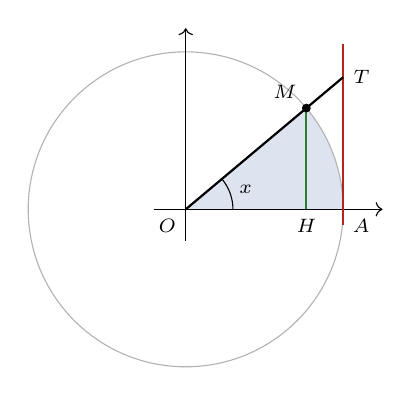
\begin{tikzpicture}[scale=2,font=\scriptsize]
\fill[cDef!15] (0,0)--(1,0) arc(0:40:1)--cycle;
\draw[gray!60] (0,0) circle(1);
\draw[->] (-0.2,0)--(1.25,0); \draw[->] (0,-0.2)--(0,1.15);
\draw[thick,cThm] (1,-0.1)--(1,1.05);
\draw[thick] (0,0)--(1,0.839) node[right]{$T$};
\draw[cRem,thick] (0.766,0)--(0.766,0.643);
\fill (0.766,0.643) circle(0.8pt) node[above left]{$M$};
\node[below left] at (0,0){$O$}; \node[below right] at (1,0){$A$}; \node[below] at (0.766,0){$H$};
\draw (0.3,0) arc(0:40:0.3); \node at (0.38,0.13){$x$};
\end{tikzpicture}\end{LTR}\end{center}}{0.58}{مساحة المثلث $OAM$ \ $\leqslant$ \ مساحة القطاع $OAM$ \ $\leqslant$ \ مساحة المثلث $OAT$:
\[\frac{\sin x}2\leqslant\frac x2\leqslant\frac{\tan x}2\]
أي: \ $\sin x\leqslant x\leqslant\dfrac{\sin x}{\cos x}$. \ بما أن $\sin x>0$ و $\cos x>0$:
\[\cos x\leqslant\frac{\sin x}x\leqslant1\]
و $\Lm{0}\cos x=1$ ، ومنه حسب الحصر: $\Lmm{0}{x>0}\dfrac{\sin x}x=1$.}
والدالة $x\mapsto\dfrac{\sin x}x$ زوجية ، إذن النهاية نفسها من اليسار: \quad \bx{\lim_{x\to0}\frac{\sin x}x=1}\par
\textbf{نتيجة:} \quad $\dfrac{\cos x-1}x=\dfrac{\cos^2x-1}{x(\cos x+1)}=-\dfrac{\sin x}x\times\dfrac{\sin x}{\cos x+1}$
\LD{\dfrac{\cos x-1}x}{0}{0} $\Car{\Lm{0}\dfrac{\sin x}x=1\\[2pt]\Lm{0}\dfrac{\sin x}{\cos x+1}=\dfrac02=0}$}{30 د}{رسم الدائرة المثلثية.}
\Row{}{%
\textbf{تطبيق: مشتقتا الدالتين $\sin$ و $\cos$:} \ من أجل $h\neq0$:
\[\frac{\sin(x+h)-\sin x}h=\sin x\times\frac{\cos h-1}h+\cos x\times\frac{\sin h}h\]
\par لدينا: $\displaystyle\lim_{h\to0}\frac{\sin(x+h)-\sin x}h=\bx{\cos x}$ لأنّ: \quad $\Car{\displaystyle\lim_{h\to0}\frac{\cos h-1}h=0\\[2pt]\displaystyle\lim_{h\to0}\frac{\sin h}h=1}$
\[\frac{\cos(x+h)-\cos x}h=\cos x\times\frac{\cos h-1}h-\sin x\times\frac{\sin h}h\]
وبنفس الطريقة النهاية لما $h\to0$ تساوي \bx{-\sin x}. \ إذن: \quad $\LW{(\sin x)^{\prime}=\cos x}$ \quad ؛ \quad $\LW{(\cos x)^{\prime}=-\sin x}$\par
\Lab{cThm}{النهايات المثلثية الشهيرة}\ ($\alpha\neq0$ ، $\beta\neq0$)
\begin{center}\begin{LTR}\renewcommand{\arraystretch}{1.9}\small
\begin{tabular}{|c|c|c|c|c|c|c|}\hline
$\dfrac{1-\cos x}{x^2}$ & $\dfrac{1-\cos x}x$ & $\dfrac{\tan\alpha x}{\tan\beta x}$ & $\dfrac{\sin\alpha x}{\sin\beta x}$ & $\dfrac{\tan x}x$ & $\dfrac{\sin x}x$ & \cellcolor{cSec!12}\ar{الدالة}\\\hline
$\LW{\dfrac12}$ & $\LW{0}$ & $\LW{\dfrac\alpha\beta}$ & $\LW{\dfrac\alpha\beta}$ & $\LW{1}$ & $\LW{1}$ & \cellcolor{cSec!12}\ar{النهاية عند $0$}\\\hline
\end{tabular}\end{LTR}\end{center}
مثلًا: \ $\dfrac{1-\cos x}{x^2}=\dfrac{\sin^2x}{x^2(1+\cos x)}=\left(\dfrac{\sin x}x\right)^2\times\dfrac1{1+\cos x}$ \ تؤول إلى $1\times\dfrac12=\dfrac12$.}{}{يُنقل الجدول في الكراس.}
\Row{التقويم}{%
\Lab{cEx}{تطبيق 3}\ احسب:\par (أ) $\Lm{0}\dfrac{\sin3x}x$ \qquad (ب) $\Lm{0}\dfrac{1-\cos x}{x\cos x}$ \qquad (جـ) $\Lm{0}\dfrac{3\sin x}{\tan x}$ \qquad (د) $\Lm{\frac\pi2}\dfrac{\cos^2x}{1-\sin x}$\par
\textbf{الحل:} (أ) نكتب: \ $\dfrac{\sin3x}x=3\times\dfrac{\sin3x}{3x}$
\LD{\dfrac{\sin3x}x}{0}{3} $\Car{\Lm{0}3x=0\\[2pt]\displaystyle\lim_{X\to0}\frac{\sin X}X=1}$
(ب) نكتب: \ $\dfrac{1-\cos x}{x\cos x}=\dfrac{1-\cos x}x\times\dfrac1{\cos x}$
\LD{\dfrac{1-\cos x}{x\cos x}}{0}{0} $\Car{\Lm{0}\dfrac{1-\cos x}x=0\\[2pt]\Lm{0}\dfrac1{\cos x}=1}$
(جـ) نكتب: \ $\dfrac{3\sin x}{\tan x}=\dfrac{3\sin x\cos x}{\sin x}=3\cos x$ \ ($x\neq0$ قريب من $0$)
\LD{\dfrac{3\sin x}{\tan x}}{0}{3} $\Car{\Lm{0}\cos x=1}$
(د) نكتب: \ $\dfrac{\cos^2x}{1-\sin x}=\dfrac{1-\sin^2x}{1-\sin x}=\dfrac{(1-\sin x)(1+\sin x)}{1-\sin x}=1+\sin x$
\LD{\dfrac{\cos^2x}{1-\sin x}}{\frac\pi2}{2} $\Car{\Lm{\frac\pi2}\sin x=1}$
\par\smallskip\textbf{ملاحظات حول سير الحصة:} \dotfill}{40 د}{تقويم فردي.}
\end{Sayr}
\end{document}
